\subsection{The five color theorem}
A weaker variant of the four color theorem is the five color theorem. It simply states that every planar graph can be colored in at most five colors instead of four.

\begin{theorem}
    Every planar graph can be colored in at most five colors.
\end{theorem}

\begin{proof}
Given a planar graph $G$. Because $G$ is planar, a known result in graph theory is that $G$ has a vertex with at most five edges. That is, there is a $v$ such that $deg(v) \leq 5$. If we can always free up a color for $v$ regardless of the colors of its neighbors, then we may simply ignore $v$ for now and color the smaller graph $G-v$ first. By repeating the same argument on $G-v$ and so on, we will eventually be left with just a single vertex. From there we can build up the 5-coloring of our graph.

Therefore, let us show that we can always free up a color for $v$. We consider two cases for $\deg(v) \leq 5$.

\begin{itemize}
    \item $\deg(v) \leq 4$. In this case, our vertex has at most four neighbors. These four neighbors have at most four different colors. This means that one color is free to be used for $v$.
    \item $\deg(v) = 5$. In this case, we have exactly five neighbors. Should our neighbors require only four colors, we can simply use our fifth color here. However, it might occur that all five neighbors use all five colors. Now we must try to free up a color in these neighbors.
\end{itemize}

Indeed, to treat the case $\deg(v)=5$ we should make a sketch of the situation first.

\begin{figure}[!h]
    \centering
    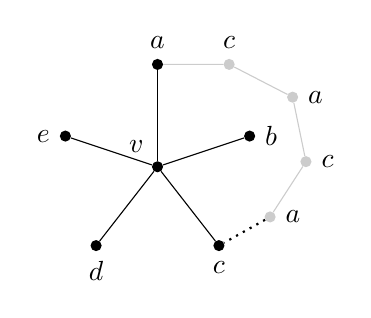
\begin{tikzpicture}[scale=1.3]
        \node[circle, fill, scale=0.015cm, label=above left:$v$] (c) at (0, 0) {};
        \node[circle, fill, scale=0.015cm, label=above:$a$] (l1) at (0, 1) { };
        \node[circle, fill, scale=0.015cm, label=right:$b$] (l2) at (0.9, 0.30) { };
        \node[circle, fill, scale=0.015cm, label=below:$c$] (l3) at (0.6, -0.77) {};
        \node[circle, fill, scale=0.015cm, label=below:$d$] (l4) at (-0.6, -0.77) {};
        \node[circle, fill, scale=0.015cm, label=left:$e$] (l5) at (-0.9, 0.30) {};
        \node[circle, fill, scale=0.015cm, label=above:$c$, opacity=0.2] (c1) at (0.7, 1) {};
        \node[circle, fill, scale=0.015cm, label=right:$a$, opacity=0.2] (c2) at (1.32, 0.68) {};
        \node[circle, fill, scale=0.015cm, label=right:$c$, opacity=0.2] (c3) at (1.45, 0.05) {};
        \node[circle, fill, scale=0.015cm, label=right:$a$, opacity=0.2] (c4) at (1.1, -0.49) {};

        \draw (c) -- (l1);
        \draw (c) -- (l2);
        \draw (c) -- (l3);
        \draw (c) -- (l4);
        \draw (c) -- (l5);

        \draw[opacity=0.2] (l1) -- (c1) -- (c2) -- (c3) -- (c4);
        \draw[dotted, thick] (c4) -- (l3);
        
    \end{tikzpicture}
    \label{fig:5colthm}
    \caption{The vertex $v$ when having five differently colored neighbors. In gray, an example $ac$-chain starting from the neighbor $a$. }
\end{figure}

Now we must ask ourselves, do these neighbors really need to use all five colors?
We may flip all the vertices colored $a$ or $c$ that are connected to the top neighbor $a$ to change its color to $c$. This way we freed up the color $a$. We say that we flipped the $ac$\textit{-chain} of neighbor $a$. Such a chain can be seen in Figure \ref{fig:5colthm}.

However, if the neighbor $c$ is part of this $ac$-chain (represented by a dotted line), then it will get flipped to $a$. So in this case we have not freed up the color $a$. We did however, isolate the vertex $b$ with the $ac$-chain. It is now impossible for a $bd$-chain from $b$ to $d$ to exist. Therefore we can flip the $bd$-chain of  $b$ to change its color into $d$ without affecting the neighbor $d$. This frees up the color $b$.

Therefore, all cases show that a color can be freed up for $v$. By our earlier argument the graph is 5-colorable.
\end{proof}
